\documentclass[11pt]{article}
\usepackage[a4paper,margin=25mm,marginparwidth=20mm,marginparsep=10pt]{geometry}
\usepackage{fontspec}
\usepackage{amsmath,amssymb,mathtools}
\usepackage{unicode-math}
\usepackage[normalem]{ulem}
\usepackage{graphicx,xcolor,tikz,tikz-cd,pdflscape,needspace}
\usetikzlibrary{calc,decorations.pathmorphing,decorations.pathreplacing,arrows.meta,shapes.geometric}
\usepackage{newunicodechar,luacode,xurl}
\usepackage[hidelinks,unicode,hypertexnames=false]{hyperref}
\setmainfont{Latin Modern Roman}
\setmathfont{Latin Modern Math}
\setmathfont{STIX Two Math}[range={"27CB,"27CD}]
% Source boldsymbol calls all request Gamma; restore its actual bold glyph.
\renewcommand\boldsymbol[1]{\symbf{#1}}
\newfontfamily\cyrfont{STIX Two Text}[Scale=MatchLowercase]
\newunicodechar{А}{{\cyrfont\char"0410}}
\newunicodechar{Б}{{\cyrfont\char"0411}}
\newunicodechar{В}{{\cyrfont\char"0412}}
\newunicodechar{Г}{{\cyrfont\char"0413}}
\newunicodechar{Д}{{\cyrfont\char"0414}}
\newunicodechar{Е}{{\cyrfont\char"0415}}
\newunicodechar{Ж}{{\cyrfont\char"0416}}
\newunicodechar{З}{{\cyrfont\char"0417}}
\newunicodechar{И}{{\cyrfont\char"0418}}
\newunicodechar{Й}{{\cyrfont\char"0419}}
\newunicodechar{К}{{\cyrfont\char"041A}}
\newunicodechar{Л}{{\cyrfont\char"041B}}
\newunicodechar{М}{{\cyrfont\char"041C}}
\newunicodechar{Н}{{\cyrfont\char"041D}}
\newunicodechar{О}{{\cyrfont\char"041E}}
\newunicodechar{П}{{\cyrfont\char"041F}}
\newunicodechar{Р}{{\cyrfont\char"0420}}
\newunicodechar{С}{{\cyrfont\char"0421}}
\newunicodechar{Т}{{\cyrfont\char"0422}}
\newunicodechar{У}{{\cyrfont\char"0423}}
\newunicodechar{Ф}{{\cyrfont\char"0424}}
\newunicodechar{Х}{{\cyrfont\char"0425}}
\newunicodechar{Ц}{{\cyrfont\char"0426}}
\newunicodechar{Ч}{{\cyrfont\char"0427}}
\newunicodechar{Ш}{{\cyrfont\char"0428}}
\newunicodechar{Щ}{{\cyrfont\char"0429}}
\newunicodechar{Ъ}{{\cyrfont\char"042A}}
\newunicodechar{Ы}{{\cyrfont\char"042B}}
\newunicodechar{Ь}{{\cyrfont\char"042C}}
\newunicodechar{Э}{{\cyrfont\char"042D}}
\newunicodechar{Ю}{{\cyrfont\char"042E}}
\newunicodechar{Я}{{\cyrfont\char"042F}}
\newunicodechar{а}{{\cyrfont\char"0430}}
\newunicodechar{б}{{\cyrfont\char"0431}}
\newunicodechar{в}{{\cyrfont\char"0432}}
\newunicodechar{г}{{\cyrfont\char"0433}}
\newunicodechar{д}{{\cyrfont\char"0434}}
\newunicodechar{е}{{\cyrfont\char"0435}}
\newunicodechar{ж}{{\cyrfont\char"0436}}
\newunicodechar{з}{{\cyrfont\char"0437}}
\newunicodechar{и}{{\cyrfont\char"0438}}
\newunicodechar{й}{{\cyrfont\char"0439}}
\newunicodechar{к}{{\cyrfont\char"043A}}
\newunicodechar{л}{{\cyrfont\char"043B}}
\newunicodechar{м}{{\cyrfont\char"043C}}
\newunicodechar{н}{{\cyrfont\char"043D}}
\newunicodechar{о}{{\cyrfont\char"043E}}
\newunicodechar{п}{{\cyrfont\char"043F}}
\newunicodechar{р}{{\cyrfont\char"0440}}
\newunicodechar{с}{{\cyrfont\char"0441}}
\newunicodechar{т}{{\cyrfont\char"0442}}
\newunicodechar{у}{{\cyrfont\char"0443}}
\newunicodechar{ф}{{\cyrfont\char"0444}}
\newunicodechar{х}{{\cyrfont\char"0445}}
\newunicodechar{ц}{{\cyrfont\char"0446}}
\newunicodechar{ч}{{\cyrfont\char"0447}}
\newunicodechar{ш}{{\cyrfont\char"0448}}
\newunicodechar{щ}{{\cyrfont\char"0449}}
\newunicodechar{ъ}{{\cyrfont\char"044A}}
\newunicodechar{ы}{{\cyrfont\char"044B}}
\newunicodechar{ь}{{\cyrfont\char"044C}}
\newunicodechar{э}{{\cyrfont\char"044D}}
\newunicodechar{ю}{{\cyrfont\char"044E}}
\newunicodechar{я}{{\cyrfont\char"044F}}
\newunicodechar{≃}{\ensuremath{\simeq}}
\newattribute\LMattr
\newcount\LMform
\newcount\LMinApp
\LMform=0
\LMinApp=0
\newcommand\LMlanguage{fr}
\newcommand\LMcotename{}
\newcommand\LMcote[1]{\gdef\LMcotename{#1}}
\newcommand\LMnotelabel{Note marginale}
\newcommand\LMappheading{Apparat du scan}
\newcommand\LMdoubtheading{Doutes conservés dans les passages biffés}
\newcommand\LMmanuscriptlabel{Manuscrit}
\newcommand\LMcorrectedlabel{Texte}
\newcommand\LMreasonlabel{Motif}
\newcommand\LMomittedlabel{omis}
\newcommand\LMinsertedlabel{ajout intégré}
\newcommand\LMlayoutlabel{Diagramme continué sur la page en paysage}
\newcommand\LMvarref[1]{\ifmmode\else\ifinner\else\textsuperscript{\textcolor{gray}{\LMreftext{#1}}}\fi\fi}
\newcommand\LMreftext[1]{\directlua{LM.reftext("\luaescapestring{#1}")}}
\newcommand\var[4]{\ifcase\LMform #1\or #2\ifnum\LMinApp=0\LMvarref{#4}\fi\or #2\fi}
\newcommand\LMadded[1]{{\color{teal}#1}}
\newcommand\deleted[1]{{\color{gray}#1}}
\newcommand\inserted[1]{{\color{teal}#1}}
\newcommand\LMarchivefooter[3]{#2}
\newcommand\LMsourceid{}
\newcommand\LMsourceMark[2]{{\def\LMsourceid{#1}#2}}
\newcommand\LMmark[1]{\directlua{LM.mark("#1",tex.inputlineno)}}
\newcommand\unsure[1]{{\color{blue}\LMmark{unsure}#1}}
\newcommand\illegible[1]{{\LMmark{illegible}\textcolor{red}{[illeg.~#1]}}}
\newcommand\LMuncertaindeletion[1]{{\color{blue}\LMmark{cancelled-anchor}\ensuremath{\dagger}}}
\newcommand\LMdoubtcopy[1]{{\color{blue}\LMmark{residual-unsure}#1}}
\newcommand\LMdoubtdata[1]{}
\newcommand\LMcancelledDoubts[1]{\ifnum\LMform=2{\color{blue}\LMmark{cancelled-anchor}\ensuremath{\dagger}}\fi}
\newcommand\scanpage[1]{%
 \par\LMflushnotes\LMflushpages\smallskip\directlua{LM.at("\luaescapestring{\LMcotename}","\luaescapestring{\detokenize{#1}}")}%
 \ifnum\LMform=2\noindent\marginpar{\footnotesize\raggedright\LMmark{scan}\textcolor{gray}{[scan #1]}}%
 \else\noindent{\footnotesize\LMmark{scan}\textcolor{gray}{[scan #1]}}\par\nobreak\fi}
\newcommand\mspage[1]{\ifnum\LMform=2\ifinner\LMqueuepage{#1}\else\marginpar{\footnotesize\raggedright\textcolor{gray}{[p.~#1]}}\fi\else{\footnotesize\textcolor{gray}{[p.~#1]}}\ \fi}
\newcommand\diagram[1]{\ifmmode\vcenter{\hbox{#1}}\else\ifinner #1\else\par\begin{center}#1\end{center}\par\LMflushnotes\LMflushpages\fi\fi}
\let\figure\relax\newcommand\figure[1]{\ifmmode\vcenter{\hbox{#1}}\else\ifinner #1\else\par\begin{center}#1\end{center}\par\LMflushnotes\LMflushpages\fi\fi}
\newcommand\LMpagefigure[2]{\ifnum\LMform=2\marginpar{\footnotesize\raggedright\textcolor{gray}{\textcircled{#2}}}\else#1\fi}
\newcommand\LMmathnotice[1]{\par\noindent{\footnotesize\color{gray}[\ensuremath{\hookrightarrow}\ #1]}\par}
\newcommand\LMlayoutnotice[1]{\par\noindent{\footnotesize\color{gray}[\LMlayoutlabel; #1]}\par}
\tolerance=1200
\emergencystretch=3em
\tracinglostchars=3
\hfuzz=0pt
\vfuzz=0pt
\raggedbottom
\renewcommand\contentsname{Sommaire}
\setcounter{tocdepth}{1}
\setlength\parindent{1.3em}
\setlength\parskip{1.5pt plus 1pt}
\allowdisplaybreaks[2]
\begin{luacode*}
-- Marked passages are linked at shipout, including paragraphs and mathematics.
-- No node, line, display or font is scaled by this code.
LM = {measure=false, maxw=0, markers={}, links=0, pages=0, scanmap={}, trial_overfull=0, shortnotes=0, blocknotes=0}
local F=LM
local A=luatexbase.registernumber('LMattr')
local HLIST,VLIST,GLUE,KERN,WHATSIT,GLYPH,PENALTY,MATH = node.id('hlist'),node.id('vlist'),node.id('glue'),node.id('kern'),node.id('whatsit'),node.id('glyph'),node.id('penalty'),node.id('math')
local STARTLINK,ENDLINK,ACTION=node.subtype('pdf_start_link'),node.subtype('pdf_end_link'),node.subtype('pdf_action')
local inert={[GLUE]=true,[KERN]=true,[PENALTY]=true,[WHATSIT]=true,[MATH]=true}
function F.at(cote,scan)
 F.cote=cote;F.scan=tonumber(string.match(scan,'^%s*(%d+)')) or 0
end
F.by_source={}
function F.mark(kind,line)
 if F.measure or not F.cote or not F.scan or F.scan==0 then return end
 local parent=tex.attribute[A]
 if not parent or parent<1 then parent=0 end
 local source=token.get_macro('LMsourceid') or ''
 if source=='' then source='auto:'..kind..':'..F.cote..':'..F.scan..':'..line end
 local id=F.by_source[source]
 if not id then
  id=#F.markers+1;F.by_source[source]=id
  F.markers[id]={id=id,source=source,kind=kind,cote=F.cote,scan=F.scan,line=line,parent=parent,runs=0,pages={},expansions=0}
 end
 local mark=F.markers[id]
 if parent~=id then mark.parent=parent end
 mark.expansions=mark.expansions+1
 tex.attribute[A]=id
end
local function url(m)
 return 'https://grothendieck.umontpellier.fr/web/viewer.html?file=../'..m.cote..'.pdf#page='..m.scan
end
local function collect(n,ids)
 local v=node.has_attribute(n,A)
 if v and v>0 then ids[v]=true end
 if (n.id==HLIST or n.id==VLIST) and n.head then for q in node.traverse(n.head) do collect(q,ids) end end
end
local function cover(id)
 local m=F.markers[id]
 if not m then return end
 m.runs=m.runs+1;m.pages[F.pages]=true
 local key=m.cote..':'..m.scan
 F.scanmap[key]=F.scanmap[key] or {};F.scanmap[key][F.pages]=true
 if m.parent>0 then cover(m.parent) end
end
local link_lists
local function link_runs(box)
 local n=box.head
 while n do
  local v=node.has_attribute(n,A)
  if v and v>0 and F.markers[v] and not inert[n.id] then
   local last,m=n,n.next
   while m do
    if inert[m.id] then
    elseif node.has_attribute(m,A)==v then last=m
    else break end
    m=m.next
   end
   local ids={};local q=n
   while q do collect(q,ids);if q==last then break end;q=q.next end
   local sorted={};for id in pairs(ids) do sorted[#sorted+1]=id;cover(id) end;table.sort(sorted)
   local w,h,d=node.dimensions(box.glue_set,box.glue_sign,box.glue_order,n,last.next)
   local s=node.new(WHATSIT,STARTLINK);s.width=w;s.height=h;s.depth=d
   local a=node.new(WHATSIT,ACTION);a.action_type=3
   a.data='/Subtype/Link/Border[0 0 0]/NM(LM'..table.concat(sorted,',')..')/A<</Type/Action/S/URI/URI('..url(F.markers[v])..')>>'
   s.action=a
   local e=node.new(WHATSIT,ENDLINK)
   box.head=node.insert_before(box.head,n,s);node.insert_after(box.head,last,e)
   F.links=F.links+1;n=e.next
  else
   if n.id==HLIST then link_runs(n) elseif n.id==VLIST then link_lists(n) end
   n=n.next
  end
 end
end
link_lists=function(box)
 for n in node.traverse(box.head) do
  if n.id==HLIST then link_runs(n) elseif n.id==VLIST then link_lists(n) end
 end
end
luatexbase.add_to_callback('pre_shipout_filter',function(box)
 F.pages=F.pages+1
 if box.id==HLIST then link_runs(box) elseif box.id==VLIST then link_lists(box) end
 return true
end,'lm.scanlinks')
-- Only discarded margin trials are measured; actual pages are never fitted.
luatexbase.add_to_callback('post_linebreak_filter',function(head)
 if F.measure then
  for line in node.traverse_id(HLIST,head) do
   if line.head then
    local nw=node.dimensions(line.glue_set,line.glue_sign,line.glue_order,line.head)
    if nw>F.maxw then F.maxw=nw end
   end
  end
 end
 return head
end,'lm.measure.margin')
-- hpack_quality replaces the engine's reporter; every actual overfull is
-- reported, with its exact width and input lines. Discarded trials are separate.
luatexbase.add_to_callback('hpack_quality',function(incident,detail,head,first,last)
 if incident=='overfull' then
  if F.measure then F.trial_overfull=F.trial_overfull+1
  else texio.write_nl('term and log',string.format('Overfull \\hbox (%.5fpt too wide) at lines %d--%d',detail/65536,first,last)) end
 elseif incident=='underfull' and not F.measure and detail>=1000 then
  texio.write_nl('log',string.format('Underfull \\hbox (badness %d) at lines %d--%d',detail,first,last))
 end
end,'lm.quality.report')
function F.summary()
 local f=assert(io.open(tex.jobname..'.lm-links.tsv','w'))
 f:write('marker\tkind\tcote\tscan\ttex_line\tparent\tlinked_runs\tphysical_pages\tsource_id\texpansions\n')
 local missing=0
 for _,m in ipairs(F.markers) do
  local ps={};for p in pairs(m.pages) do ps[#ps+1]=p end;table.sort(ps)
  if m.runs==0 then missing=missing+1 end
  f:write(table.concat({m.id,m.kind,m.cote,m.scan,m.line,m.parent,m.runs,table.concat(ps,','),m.source,m.expansions},'\t'),'\n')
 end
 f:close()
 local g=assert(io.open(tex.jobname..'.lm-scans.tsv','w'));g:write('cote\tscan\tphysical_pages\tsource_id\texpansions\n')
 local ks={};for k in pairs(F.scanmap) do ks[#ks+1]=k end;table.sort(ks)
 for _,k in ipairs(ks) do
  local cote,scan=string.match(k,'(.*):(%d+)');local ps={};for p in pairs(F.scanmap[k]) do ps[#ps+1]=p end;table.sort(ps)
  g:write(cote,'\t',scan,'\t',table.concat(ps,','),'\n')
 end;g:close()
 texio.write_nl('term and log',string.format('LM-AUDIT markers=%d links=%d unlinked=%d scans=%d pages=%d margin_short=%d margin_block=%d discarded_trial_overfull=%d',#F.markers,F.links,missing,#ks,F.pages,F.shortnotes,F.blocknotes,F.trial_overfull))
end

function LM.reftext(s)
 local a,b=string.match(s,'([A-Z])0*(%d+)$')
 tex.sprint(a and (string.lower(a)..b) or '*')
end

LM.noteids={};LM.nextnote=0;LM.pageids={}
function LM.noteref(source)
 if source=='' then source='note:'..tex.inputlineno end
 local id=LM.noteids[source]
 local fresh=0
 if not id then LM.nextnote=LM.nextnote+1;id=LM.nextnote;LM.noteids[source]=id;fresh=1 end
 tex.sprint('\\def\\LMcurrentnoteref{'..id..'}\\LMnotefresh='..fresh..'\\relax')
end
function LM.pagequeue(source)
 local fresh=0
 if not LM.pageids[source] then LM.pageids[source]=true;fresh=1 end
 tex.count.LMnotefresh=fresh
end

\end{luacode*}
\makeatletter
\AtBeginDocument{\let\LMsimeq\simeq\protected\def\simeq{\ifmmode\LMsimeq\else$\LMsimeq$\fi}%
 \let\LMGamma\Gamma\protected\def\Gamma{\ifmmode\LMGamma\else$\LMGamma$\fi}}
\output\expandafter{\expandafter\unsetattribute\expandafter\LMattr\the\output}
\AtEndDocument{\clearpage\directlua{LM.summary()}}
\newif\ifLMtrial
\newcount\LMnotefresh
\newcommand\LMcurrentnoteref{}
\newcommand\LMgetnoteref{\directlua{LM.noteref("\luaescapestring{\LMsourceid}")}}
\newsavebox\LMmbox
\newdimen\LMmw
\newdimen\LMmh
\newdimen\LMnotewidth
\newcommand\LMmarginstyle{\footnotesize\rightskip=0pt plus 2.5em\relax\parfillskip=0pt plus 1fil\relax\hyphenpenalty=50\relax\def\margin##1{{[##1]}}}
\newcommand\LMtrial[2]{%
 \LMtrialtrue\directlua{LM.measure=true LM.maxw=0}%
 \setbox\LMmbox\vbox{\hsize=#1\relax\@parboxrestore\LMmarginstyle #2\par}%
 \LMtrialfalse\directlua{LM.measure=false tex.setdimen("LMmw",LM.maxw)}%
 \LMmh=\dimexpr\ht\LMmbox+\dp\LMmbox\relax}
\newcommand\LMinblock[1]{%
 \directlua{LM.blocknotes=LM.blocknotes+1}%
 \par\smallskip\noindent{\color{gray}\rule{.20\linewidth}{.35pt}}\par\nobreak
 \begingroup\LMmarginstyle\parindent=0pt\@beginparpenalty=10000\relax
 \noindent\textit{\LMnotelabel.}\enspace #1\par\endgroup\smallskip}
\newcommand\LMmargin[1]{\begingroup\LMgetnoteref
 \LMtrial{\marginparwidth}{#1}%
 \ifdim\LMmw>\marginparwidth\LMnotemark{\LMcurrentnoteref}\LMinblock{\textsuperscript{m\LMcurrentnoteref}\ #1}%
 \else\ifdim\LMmh>33pt\LMnotemark{\LMcurrentnoteref}\LMinblock{\textsuperscript{m\LMcurrentnoteref}\ #1}%
 \else\directlua{LM.shortnotes=LM.shortnotes+1}\marginpar{\LMmarginstyle #1}%
 \fi\fi\endgroup}
% This source-local wrapper retains both consecutive short notes on separate lines.
\newcommand\LMpairedmargins[1]{\begingroup
 \marginpar{\LMmarginstyle
  \def\margin##1{\LMgetnoteref\directlua{LM.shortnotes=LM.shortnotes+1}\noindent##1\par}#1}%
 \endgroup}
\newcounter{LMnoteref}
\newcommand\LMpendingnotes{}
\newcommand\LMpendingpages{}
\newcommand\LMqueuepage[1]{\ifLMtrial\else\directlua{LM.pagequeue("\luaescapestring{\LMsourceid}")}\ifnum\LMnotefresh=1\g@addto@macro\LMpendingpages{\marginpar{\footnotesize\raggedright\textcolor{gray}{[p.~#1]}}}\fi\fi}
\newcommand\LMflushpages{\ifinner\else\LMpendingpages\global\let\LMpendingpages\@empty\fi}
\newcommand\LMnotemark[1]{\ifmmode{}^{\scriptscriptstyle\text{\color{gray}m#1}}\else\textsuperscript{\color{gray}m#1}\fi}
\newcommand\LMqueuenote[1]{%
 \LMgetnoteref\LMnotemark{\LMcurrentnoteref}%
 \ifnum\LMnotefresh=1\begingroup\edef\LMnext{\endgroup\noexpand\g@addto@macro\noexpand\LMpendingnotes{\noexpand\LMqueuednote{\LMcurrentnoteref}{\the\LMattr}{\unexpanded{#1}}}}\LMnext\fi}
\newcommand\LMqueuednote[3]{\begingroup\LMattr=#2\relax\ifnum#2>0\color{blue}\fi\LMinblock{\textsuperscript{m#1}\ #3}\endgroup}
\newcommand\LMflushnotes{\ifinner\else\begingroup\let\LMnextnotes\LMpendingnotes\global\let\LMpendingnotes\@empty\LMnextnotes\endgroup\fi}
\newcommand\margin[1]{\ifmmode\LMqueuenote{\(#1\)}\else\ifinner\LMqueuenote{#1}\else\LMmargin{#1}\fi\fi}
\AddToHook{env/equation*/after}{\LMflushnotes\LMflushpages}
\AddToHook{env/equation/after}{\LMflushnotes\LMflushpages}
\AddToHook{env/align*/after}{\LMflushnotes\LMflushpages}
\AddToHook{env/align/after}{\LMflushnotes\LMflushpages}
\AddToHook{env/gather*/after}{\LMflushnotes\LMflushpages}
\AddToHook{env/center/after}{\LMflushnotes\LMflushpages}
\makeatother
\newenvironment{LMapparatus}{\par\smallskip\begingroup\LMinApp=1\footnotesize\noindent\textcolor{gray}{\rule{.26\linewidth}{.35pt}}\par\noindent\textbf{\LMappheading}\par\smallskip}{\par\endgroup}
\newcommand\LMentry[6]{\par\noindent{\color{gray}\texttt{#1}}\enspace\textit{#2.}\enspace\textit{\LMmanuscriptlabel:}\enspace #3\par\noindent\textit{\LMcorrectedlabel:}\enspace #4\enspace\textit{\LMreasonlabel:}\enspace #5\par\smallskip}
\newcommand\LMcarryover[2]{\par\noindent{\scriptsize\color{gray}\texttt{#1}}\enspace #2\par}

\begin{document}\LMcote{140-2}
\clearpage\noindent Probe 582 preceding material.\par
\noindent Ordinary preceding paragraph line 1.\par
\noindent Ordinary preceding paragraph line 2.\par
\noindent Ordinary preceding paragraph line 3.\par
\noindent Ordinary preceding paragraph line 4.\par
\noindent Ordinary preceding paragraph line 5.\par
\noindent Ordinary preceding paragraph line 6.\par
\noindent Ordinary preceding paragraph line 7.\par
\noindent Ordinary preceding paragraph line 8.\par
\noindent Ordinary preceding paragraph line 9.\par
\noindent Ordinary preceding paragraph line 10.\par
\noindent Ordinary preceding paragraph line 11.\par
\noindent Ordinary preceding paragraph line 12.\par
\noindent Ordinary preceding paragraph line 13.\par
\noindent Ordinary preceding paragraph line 14.\par
\noindent Ordinary preceding paragraph line 15.\par
\noindent Ordinary preceding paragraph line 16.\par
\noindent Ordinary preceding paragraph line 17.\par
\noindent Ordinary preceding paragraph line 18.\par
\noindent Ordinary preceding paragraph line 19.\par
\noindent Ordinary preceding paragraph line 20.\par
\noindent Ordinary preceding paragraph line 21.\par
\noindent Ordinary preceding paragraph line 22.\par
\noindent Ordinary preceding paragraph line 23.\par
\noindent Ordinary preceding paragraph line 24.\par
\noindent Ordinary preceding paragraph line 25.\par
\noindent Ordinary preceding paragraph line 26.\par
\noindent Ordinary preceding paragraph line 27.\par
\noindent Ordinary preceding paragraph line 28.\par
\noindent Ordinary preceding paragraph line 29.\par
\noindent Ordinary preceding paragraph line 30.\par
\noindent Ordinary preceding paragraph line 31.\par
\noindent Ordinary preceding paragraph line 32.\par
\noindent Ordinary preceding paragraph line 33.\par
\noindent Ordinary preceding paragraph line 34.\par
\noindent Ordinary preceding paragraph line 35.\par
\noindent Ordinary preceding paragraph line 36.\par
\noindent Ordinary preceding paragraph line 37.\par
\noindent Ordinary preceding paragraph line 38.\par
\noindent Ordinary preceding paragraph line 39.\par
\noindent Ordinary preceding paragraph line 40.\par
\noindent Ordinary preceding paragraph line 41.\par
\noindent Ordinary preceding paragraph line 42.\par
\noindent Ordinary preceding paragraph line 43.\par
\LMinblock{\textsuperscript{m582} \diagram{\begin{tikzcd}[ampersand replacement=\&]
1 \arrow[r] \& \pi' \arrow[r] \arrow[d] \& \mathcal E'_K \arrow[r] \arrow[d] \& K \arrow[r,dash] \arrow[d,equal] \& 1 \\
1 \arrow[r,dash] \& \pi \arrow[r] \& \mathcal E_K \arrow[r,dash] \& K \arrow[r,dash] \& 1
\end{tikzcd}}}
\noindent End of probe 582.\par
\clearpage\noindent Probe 599 preceding material.\par
\noindent Ordinary preceding paragraph line 1.\par
\noindent Ordinary preceding paragraph line 2.\par
\noindent Ordinary preceding paragraph line 3.\par
\noindent Ordinary preceding paragraph line 4.\par
\noindent Ordinary preceding paragraph line 5.\par
\noindent Ordinary preceding paragraph line 6.\par
\noindent Ordinary preceding paragraph line 7.\par
\noindent Ordinary preceding paragraph line 8.\par
\noindent Ordinary preceding paragraph line 9.\par
\noindent Ordinary preceding paragraph line 10.\par
\noindent Ordinary preceding paragraph line 11.\par
\noindent Ordinary preceding paragraph line 12.\par
\noindent Ordinary preceding paragraph line 13.\par
\noindent Ordinary preceding paragraph line 14.\par
\noindent Ordinary preceding paragraph line 15.\par
\noindent Ordinary preceding paragraph line 16.\par
\noindent Ordinary preceding paragraph line 17.\par
\noindent Ordinary preceding paragraph line 18.\par
\noindent Ordinary preceding paragraph line 19.\par
\noindent Ordinary preceding paragraph line 20.\par
\noindent Ordinary preceding paragraph line 21.\par
\noindent Ordinary preceding paragraph line 22.\par
\noindent Ordinary preceding paragraph line 23.\par
\noindent Ordinary preceding paragraph line 24.\par
\noindent Ordinary preceding paragraph line 25.\par
\noindent Ordinary preceding paragraph line 26.\par
\noindent Ordinary preceding paragraph line 27.\par
\noindent Ordinary preceding paragraph line 28.\par
\noindent Ordinary preceding paragraph line 29.\par
\noindent Ordinary preceding paragraph line 30.\par
\noindent Ordinary preceding paragraph line 31.\par
\noindent Ordinary preceding paragraph line 32.\par
\noindent Ordinary preceding paragraph line 33.\par
\noindent Ordinary preceding paragraph line 34.\par
\noindent Ordinary preceding paragraph line 35.\par
\noindent Ordinary preceding paragraph line 36.\par
\noindent Ordinary preceding paragraph line 37.\par
\noindent Ordinary preceding paragraph line 38.\par
\noindent Ordinary preceding paragraph line 39.\par
\noindent Ordinary preceding paragraph line 40.\par
\noindent Ordinary preceding paragraph line 41.\par
\noindent Ordinary preceding paragraph line 42.\par
\noindent Ordinary preceding paragraph line 43.\par
\LMinblock{\textsuperscript{m599} \figure{\begin{tikzpicture}[x=1cm,y=1cm,line cap=round,line join=round]
\draw[line width=.45pt] (0,2.85)
 .. controls (-.71,2.83) and (-1.02,2.47) .. (-1,2)
 .. controls (-1.01,1.48) and (-.57,1.16) .. (0,1.15);
\draw[line width=.45pt] (0,2.85)
 .. controls (.76,2.85) and (1.03,2.48) .. (1,2.10);
\draw[line width=.45pt] (.99,1.98)
 .. controls (.98,1.62) and (.74,1.36) .. (.54,1.26);
\draw[line width=.5pt] (-1,2)
 .. controls (-.91,1.75) and (.83,1.74) .. (1,1.95);
\draw[densely dotted,line width=.65pt] (-1,2)
 .. controls (-.61,2.17) and (.63,2.17) .. (1,2.02);
\fill (0,2.85) circle (1.4pt);
\node[anchor=south west,inner sep=2pt] at (0,2.88) {$P=\unsure{-\bar j|-j}$};
\fill (0,1.15) circle (1.4pt);
\node[anchor=north west,inner sep=2pt] at (-.03,1.12) {$P'=\unsure{-j|-\bar j}$};
\fill (-.57,1.80) circle (1.4pt);
\node[below,inner sep=2pt] at (-.57,1.80) {$0$};
\fill (.78,1.82) circle (1.4pt);
\node[below,inner sep=2pt] at (.78,1.82) {$1$};
\fill (0,2.12) circle (1.5pt);
\node[above,inner sep=2pt] at (0,2.12) {$\infty$};
\draw[->,line width=.65pt] (-1.40,1.60)
 .. controls (-1.40,1.22) and (-1.38,.85) .. (-1.37,.58);
\draw[line width=.45pt] (.02,.48)
 .. controls (-.55,.48) and (-.86,.17) .. (-.82,-.20)
 .. controls (-.78,-.70) and (-.46,-1.02) .. (.10,-1.04);
\draw[line width=.45pt] (.02,.48)
 .. controls (.65,.46) and (.87,.12) .. (.82,-.29)
 .. controls (.81,-.58) and (.66,-.79) .. (.53,-.87);
\fill (.02,.48) circle (1.5pt);
\node[anchor=west,inner sep=2pt] at (.07,.48) {$\unsure{Q}(=P)$};
\fill (-.82,-.12) circle (1.5pt);
\node[left,inner sep=2pt] at (-.82,-.12) {$\infty$};
\fill (-.08,.10) circle (1.7pt);
\node[below,inner sep=2pt] at (-.08,.10) {$1$};
\fill (-.40,-.36) circle (1.7pt);
\node[below,inner sep=2pt] at (-.40,-.36) {$0$};
\draw[line width=1.15pt] (-.08,.10)
 .. controls (.28,.10) and (.71,.02) .. (.82,-.20)
 .. controls (.66,-.43) and (.03,-.47) .. (-.40,-.36);
\draw[densely dotted,line width=.65pt] (-.82,-.12)
 .. controls (-.60,.08) and (-.36,.08) .. (-.08,.10);
\draw[densely dotted,line width=.65pt] (-.82,-.12)
 .. controls (-.78,-.32) and (-.59,-.35) .. (-.40,-.36);
\node[below,inner sep=1pt] at (.22,-.44) {$\unsure{\varphi}$};
\end{tikzpicture}}}
\noindent End of probe 599.\par
\clearpage\noindent Probe 725 preceding material.\par
\noindent Ordinary preceding paragraph line 1.\par
\noindent Ordinary preceding paragraph line 2.\par
\noindent Ordinary preceding paragraph line 3.\par
\noindent Ordinary preceding paragraph line 4.\par
\noindent Ordinary preceding paragraph line 5.\par
\noindent Ordinary preceding paragraph line 6.\par
\noindent Ordinary preceding paragraph line 7.\par
\noindent Ordinary preceding paragraph line 8.\par
\noindent Ordinary preceding paragraph line 9.\par
\noindent Ordinary preceding paragraph line 10.\par
\noindent Ordinary preceding paragraph line 11.\par
\noindent Ordinary preceding paragraph line 12.\par
\noindent Ordinary preceding paragraph line 13.\par
\noindent Ordinary preceding paragraph line 14.\par
\noindent Ordinary preceding paragraph line 15.\par
\noindent Ordinary preceding paragraph line 16.\par
\noindent Ordinary preceding paragraph line 17.\par
\noindent Ordinary preceding paragraph line 18.\par
\noindent Ordinary preceding paragraph line 19.\par
\noindent Ordinary preceding paragraph line 20.\par
\noindent Ordinary preceding paragraph line 21.\par
\noindent Ordinary preceding paragraph line 22.\par
\noindent Ordinary preceding paragraph line 23.\par
\noindent Ordinary preceding paragraph line 24.\par
\noindent Ordinary preceding paragraph line 25.\par
\noindent Ordinary preceding paragraph line 26.\par
\noindent Ordinary preceding paragraph line 27.\par
\noindent Ordinary preceding paragraph line 28.\par
\noindent Ordinary preceding paragraph line 29.\par
\noindent Ordinary preceding paragraph line 30.\par
\noindent Ordinary preceding paragraph line 31.\par
\noindent Ordinary preceding paragraph line 32.\par
\noindent Ordinary preceding paragraph line 33.\par
\noindent Ordinary preceding paragraph line 34.\par
\noindent Ordinary preceding paragraph line 35.\par
\noindent Ordinary preceding paragraph line 36.\par
\noindent Ordinary preceding paragraph line 37.\par
\noindent Ordinary preceding paragraph line 38.\par
\noindent Ordinary preceding paragraph line 39.\par
\noindent Ordinary preceding paragraph line 40.\par
\noindent Ordinary preceding paragraph line 41.\par
\noindent Ordinary preceding paragraph line 42.\par
\noindent Ordinary preceding paragraph line 43.\par
\LMinblock{\textsuperscript{m725} \figure{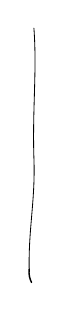
\begin{tikzpicture}[x=1cm,y=1cm,line cap=round]
\draw[line width=.30pt] (.04,0) .. controls (.08,-.55) and (.02,-1.02) .. (.04,-1.65)
 .. controls (.06,-2.18) and (-.03,-2.54) .. (-.02,-3.06);
\draw[line width=.52pt] (-.02,-3.06) .. controls (-.03,-3.13) and (-.01,-3.19) .. (.01,-3.23);
\end{tikzpicture}}}
\noindent End of probe 725.\par
\clearpage\noindent Probe 1108 preceding material.\par
\noindent Ordinary preceding paragraph line 1.\par
\noindent Ordinary preceding paragraph line 2.\par
\noindent Ordinary preceding paragraph line 3.\par
\noindent Ordinary preceding paragraph line 4.\par
\noindent Ordinary preceding paragraph line 5.\par
\noindent Ordinary preceding paragraph line 6.\par
\noindent Ordinary preceding paragraph line 7.\par
\noindent Ordinary preceding paragraph line 8.\par
\noindent Ordinary preceding paragraph line 9.\par
\noindent Ordinary preceding paragraph line 10.\par
\noindent Ordinary preceding paragraph line 11.\par
\noindent Ordinary preceding paragraph line 12.\par
\noindent Ordinary preceding paragraph line 13.\par
\noindent Ordinary preceding paragraph line 14.\par
\noindent Ordinary preceding paragraph line 15.\par
\noindent Ordinary preceding paragraph line 16.\par
\noindent Ordinary preceding paragraph line 17.\par
\noindent Ordinary preceding paragraph line 18.\par
\noindent Ordinary preceding paragraph line 19.\par
\noindent Ordinary preceding paragraph line 20.\par
\noindent Ordinary preceding paragraph line 21.\par
\noindent Ordinary preceding paragraph line 22.\par
\noindent Ordinary preceding paragraph line 23.\par
\noindent Ordinary preceding paragraph line 24.\par
\noindent Ordinary preceding paragraph line 25.\par
\noindent Ordinary preceding paragraph line 26.\par
\noindent Ordinary preceding paragraph line 27.\par
\noindent Ordinary preceding paragraph line 28.\par
\noindent Ordinary preceding paragraph line 29.\par
\noindent Ordinary preceding paragraph line 30.\par
\noindent Ordinary preceding paragraph line 31.\par
\noindent Ordinary preceding paragraph line 32.\par
\noindent Ordinary preceding paragraph line 33.\par
\noindent Ordinary preceding paragraph line 34.\par
\noindent Ordinary preceding paragraph line 35.\par
\noindent Ordinary preceding paragraph line 36.\par
\noindent Ordinary preceding paragraph line 37.\par
\noindent Ordinary preceding paragraph line 38.\par
\noindent Ordinary preceding paragraph line 39.\par
\noindent Ordinary preceding paragraph line 40.\par
\noindent Ordinary preceding paragraph line 41.\par
\noindent Ordinary preceding paragraph line 42.\par
\noindent Ordinary preceding paragraph line 43.\par
\LMinblock{\textsuperscript{m1108} \figure{\begin{tikzpicture}[x=.65cm,y=.65cm]
\draw[->] (0,4.5) .. controls (1.1,4.55) and (1.1,3.7) .. (1.1,3.25)
 -- (1.2,.8) .. controls (1.2,.45) and (1.55,.55) .. (2.4,.65);
\draw (0,0) .. controls (1.0,-.05) and (1.05,.1) .. (1.15,.45)
 .. controls (1.25,.75) and (1.55,.65) .. (2.4,.65);
\end{tikzpicture}}}
\noindent End of probe 1108.\par
\clearpage\noindent Long note must span pages.\par
\LMinblock{\textsuperscript{mLONG} Paragraph 1. This is a deliberately long marginal note. Its prose must remain breakable across pages, while the heading stays attached to its first line.\par
Paragraph 2. This is a deliberately long marginal note. Its prose must remain breakable across pages, while the heading stays attached to its first line.\par
Paragraph 3. This is a deliberately long marginal note. Its prose must remain breakable across pages, while the heading stays attached to its first line.\par
Paragraph 4. This is a deliberately long marginal note. Its prose must remain breakable across pages, while the heading stays attached to its first line.\par
Paragraph 5. This is a deliberately long marginal note. Its prose must remain breakable across pages, while the heading stays attached to its first line.\par
Paragraph 6. This is a deliberately long marginal note. Its prose must remain breakable across pages, while the heading stays attached to its first line.\par
Paragraph 7. This is a deliberately long marginal note. Its prose must remain breakable across pages, while the heading stays attached to its first line.\par
Paragraph 8. This is a deliberately long marginal note. Its prose must remain breakable across pages, while the heading stays attached to its first line.\par
Paragraph 9. This is a deliberately long marginal note. Its prose must remain breakable across pages, while the heading stays attached to its first line.\par
Paragraph 10. This is a deliberately long marginal note. Its prose must remain breakable across pages, while the heading stays attached to its first line.\par
Paragraph 11. This is a deliberately long marginal note. Its prose must remain breakable across pages, while the heading stays attached to its first line.\par
Paragraph 12. This is a deliberately long marginal note. Its prose must remain breakable across pages, while the heading stays attached to its first line.\par
Paragraph 13. This is a deliberately long marginal note. Its prose must remain breakable across pages, while the heading stays attached to its first line.\par
Paragraph 14. This is a deliberately long marginal note. Its prose must remain breakable across pages, while the heading stays attached to its first line.\par
Paragraph 15. This is a deliberately long marginal note. Its prose must remain breakable across pages, while the heading stays attached to its first line.\par
Paragraph 16. This is a deliberately long marginal note. Its prose must remain breakable across pages, while the heading stays attached to its first line.\par
Paragraph 17. This is a deliberately long marginal note. Its prose must remain breakable across pages, while the heading stays attached to its first line.\par
Paragraph 18. This is a deliberately long marginal note. Its prose must remain breakable across pages, while the heading stays attached to its first line.\par
Paragraph 19. This is a deliberately long marginal note. Its prose must remain breakable across pages, while the heading stays attached to its first line.\par
Paragraph 20. This is a deliberately long marginal note. Its prose must remain breakable across pages, while the heading stays attached to its first line.\par
Paragraph 21. This is a deliberately long marginal note. Its prose must remain breakable across pages, while the heading stays attached to its first line.\par
Paragraph 22. This is a deliberately long marginal note. Its prose must remain breakable across pages, while the heading stays attached to its first line.\par
Paragraph 23. This is a deliberately long marginal note. Its prose must remain breakable across pages, while the heading stays attached to its first line.\par
Paragraph 24. This is a deliberately long marginal note. Its prose must remain breakable across pages, while the heading stays attached to its first line.\par
Paragraph 25. This is a deliberately long marginal note. Its prose must remain breakable across pages, while the heading stays attached to its first line.\par
Paragraph 26. This is a deliberately long marginal note. Its prose must remain breakable across pages, while the heading stays attached to its first line.\par
Paragraph 27. This is a deliberately long marginal note. Its prose must remain breakable across pages, while the heading stays attached to its first line.\par
Paragraph 28. This is a deliberately long marginal note. Its prose must remain breakable across pages, while the heading stays attached to its first line.\par
Paragraph 29. This is a deliberately long marginal note. Its prose must remain breakable across pages, while the heading stays attached to its first line.\par
Paragraph 30. This is a deliberately long marginal note. Its prose must remain breakable across pages, while the heading stays attached to its first line.\par
Paragraph 31. This is a deliberately long marginal note. Its prose must remain breakable across pages, while the heading stays attached to its first line.\par
Paragraph 32. This is a deliberately long marginal note. Its prose must remain breakable across pages, while the heading stays attached to its first line.\par
Paragraph 33. This is a deliberately long marginal note. Its prose must remain breakable across pages, while the heading stays attached to its first line.\par
Paragraph 34. This is a deliberately long marginal note. Its prose must remain breakable across pages, while the heading stays attached to its first line.\par
Paragraph 35. This is a deliberately long marginal note. Its prose must remain breakable across pages, while the heading stays attached to its first line.\par
Paragraph 36. This is a deliberately long marginal note. Its prose must remain breakable across pages, while the heading stays attached to its first line.\par
Paragraph 37. This is a deliberately long marginal note. Its prose must remain breakable across pages, while the heading stays attached to its first line.\par
Paragraph 38. This is a deliberately long marginal note. Its prose must remain breakable across pages, while the heading stays attached to its first line.\par
Paragraph 39. This is a deliberately long marginal note. Its prose must remain breakable across pages, while the heading stays attached to its first line.\par
Paragraph 40. This is a deliberately long marginal note. Its prose must remain breakable across pages, while the heading stays attached to its first line.\par
Paragraph 41. This is a deliberately long marginal note. Its prose must remain breakable across pages, while the heading stays attached to its first line.\par
Paragraph 42. This is a deliberately long marginal note. Its prose must remain breakable across pages, while the heading stays attached to its first line.\par
Paragraph 43. This is a deliberately long marginal note. Its prose must remain breakable across pages, while the heading stays attached to its first line.\par
Paragraph 44. This is a deliberately long marginal note. Its prose must remain breakable across pages, while the heading stays attached to its first line.\par
Paragraph 45. This is a deliberately long marginal note. Its prose must remain breakable across pages, while the heading stays attached to its first line.\par
Paragraph 46. This is a deliberately long marginal note. Its prose must remain breakable across pages, while the heading stays attached to its first line.\par
Paragraph 47. This is a deliberately long marginal note. Its prose must remain breakable across pages, while the heading stays attached to its first line.\par
Paragraph 48. This is a deliberately long marginal note. Its prose must remain breakable across pages, while the heading stays attached to its first line.\par
Paragraph 49. This is a deliberately long marginal note. Its prose must remain breakable across pages, while the heading stays attached to its first line.\par
Paragraph 50. This is a deliberately long marginal note. Its prose must remain breakable across pages, while the heading stays attached to its first line.\par
Paragraph 51. This is a deliberately long marginal note. Its prose must remain breakable across pages, while the heading stays attached to its first line.\par
Paragraph 52. This is a deliberately long marginal note. Its prose must remain breakable across pages, while the heading stays attached to its first line.\par
Paragraph 53. This is a deliberately long marginal note. Its prose must remain breakable across pages, while the heading stays attached to its first line.\par
Paragraph 54. This is a deliberately long marginal note. Its prose must remain breakable across pages, while the heading stays attached to its first line.\par
Paragraph 55. This is a deliberately long marginal note. Its prose must remain breakable across pages, while the heading stays attached to its first line.\par
Paragraph 56. This is a deliberately long marginal note. Its prose must remain breakable across pages, while the heading stays attached to its first line.\par
Paragraph 57. This is a deliberately long marginal note. Its prose must remain breakable across pages, while the heading stays attached to its first line.\par
Paragraph 58. This is a deliberately long marginal note. Its prose must remain breakable across pages, while the heading stays attached to its first line.\par
Paragraph 59. This is a deliberately long marginal note. Its prose must remain breakable across pages, while the heading stays attached to its first line.\par
Paragraph 60. This is a deliberately long marginal note. Its prose must remain breakable across pages, while the heading stays attached to its first line.\par
Paragraph 61. This is a deliberately long marginal note. Its prose must remain breakable across pages, while the heading stays attached to its first line.\par
Paragraph 62. This is a deliberately long marginal note. Its prose must remain breakable across pages, while the heading stays attached to its first line.\par
Paragraph 63. This is a deliberately long marginal note. Its prose must remain breakable across pages, while the heading stays attached to its first line.\par
Paragraph 64. This is a deliberately long marginal note. Its prose must remain breakable across pages, while the heading stays attached to its first line.\par
Paragraph 65. This is a deliberately long marginal note. Its prose must remain breakable across pages, while the heading stays attached to its first line.\par
Paragraph 66. This is a deliberately long marginal note. Its prose must remain breakable across pages, while the heading stays attached to its first line.\par
Paragraph 67. This is a deliberately long marginal note. Its prose must remain breakable across pages, while the heading stays attached to its first line.\par
Paragraph 68. This is a deliberately long marginal note. Its prose must remain breakable across pages, while the heading stays attached to its first line.\par
Paragraph 69. This is a deliberately long marginal note. Its prose must remain breakable across pages, while the heading stays attached to its first line.\par
Paragraph 70. This is a deliberately long marginal note. Its prose must remain breakable across pages, while the heading stays attached to its first line.\par
Paragraph 71. This is a deliberately long marginal note. Its prose must remain breakable across pages, while the heading stays attached to its first line.\par
Paragraph 72. This is a deliberately long marginal note. Its prose must remain breakable across pages, while the heading stays attached to its first line.\par
Paragraph 73. This is a deliberately long marginal note. Its prose must remain breakable across pages, while the heading stays attached to its first line.\par
Paragraph 74. This is a deliberately long marginal note. Its prose must remain breakable across pages, while the heading stays attached to its first line.\par
Paragraph 75. This is a deliberately long marginal note. Its prose must remain breakable across pages, while the heading stays attached to its first line.\par
Paragraph 76. This is a deliberately long marginal note. Its prose must remain breakable across pages, while the heading stays attached to its first line.\par
Paragraph 77. This is a deliberately long marginal note. Its prose must remain breakable across pages, while the heading stays attached to its first line.\par
Paragraph 78. This is a deliberately long marginal note. Its prose must remain breakable across pages, while the heading stays attached to its first line.\par
Paragraph 79. This is a deliberately long marginal note. Its prose must remain breakable across pages, while the heading stays attached to its first line.\par
Paragraph 80. This is a deliberately long marginal note. Its prose must remain breakable across pages, while the heading stays attached to its first line.\par
Paragraph 81. This is a deliberately long marginal note. Its prose must remain breakable across pages, while the heading stays attached to its first line.\par
Paragraph 82. This is a deliberately long marginal note. Its prose must remain breakable across pages, while the heading stays attached to its first line.\par
Paragraph 83. This is a deliberately long marginal note. Its prose must remain breakable across pages, while the heading stays attached to its first line.\par
Paragraph 84. This is a deliberately long marginal note. Its prose must remain breakable across pages, while the heading stays attached to its first line.\par
Paragraph 85. This is a deliberately long marginal note. Its prose must remain breakable across pages, while the heading stays attached to its first line.\par
Paragraph 86. This is a deliberately long marginal note. Its prose must remain breakable across pages, while the heading stays attached to its first line.\par
Paragraph 87. This is a deliberately long marginal note. Its prose must remain breakable across pages, while the heading stays attached to its first line.\par
Paragraph 88. This is a deliberately long marginal note. Its prose must remain breakable across pages, while the heading stays attached to its first line.\par
Paragraph 89. This is a deliberately long marginal note. Its prose must remain breakable across pages, while the heading stays attached to its first line.\par
Paragraph 90. This is a deliberately long marginal note. Its prose must remain breakable across pages, while the heading stays attached to its first line.\par
Paragraph 91. This is a deliberately long marginal note. Its prose must remain breakable across pages, while the heading stays attached to its first line.\par
Paragraph 92. This is a deliberately long marginal note. Its prose must remain breakable across pages, while the heading stays attached to its first line.\par
Paragraph 93. This is a deliberately long marginal note. Its prose must remain breakable across pages, while the heading stays attached to its first line.\par
Paragraph 94. This is a deliberately long marginal note. Its prose must remain breakable across pages, while the heading stays attached to its first line.\par
Paragraph 95. This is a deliberately long marginal note. Its prose must remain breakable across pages, while the heading stays attached to its first line.\par
Paragraph 96. This is a deliberately long marginal note. Its prose must remain breakable across pages, while the heading stays attached to its first line.\par
Paragraph 97. This is a deliberately long marginal note. Its prose must remain breakable across pages, while the heading stays attached to its first line.\par
Paragraph 98. This is a deliberately long marginal note. Its prose must remain breakable across pages, while the heading stays attached to its first line.\par
Paragraph 99. This is a deliberately long marginal note. Its prose must remain breakable across pages, while the heading stays attached to its first line.\par
Paragraph 100. This is a deliberately long marginal note. Its prose must remain breakable across pages, while the heading stays attached to its first line.\par}
\end{document}
